\chapter{Sound-wave characterization}
\label{app:SoundWaveCharacterization}
Sound waves have the well-known dispersion relation
\begin{equation}
  \omega = c_s k,
  \label{eq:SoundWaveCharacterization:sound_wave_dispersion_relation}
\end{equation}
where
$\omega$ is the angular frequency of the sound wave,
$k$ is the wavenumber of the sound wave, and
$c_s = \SI{343}{\meter\per\second}$ is the sound speed
in dry air at sea level and $T = \SI{20}{\celsius}$.
Further, the sound-wave pressure fluctuations
produce corresponding fluctuations in the refractive index,
making sound waves an ideal tool
for probing the wavenumber response of an interferometer.
A quantitative comparison between
the predicted and observed interferometer responses, however,
requires an accurate description of the sound-wave pressure fluctuations.

It is the intent of this appendix
to quantitatively characterize the sound-wave pressure fluctuations
driven by the speaker used throughout this thesis.
Below, Section~\ref{sec:SoundWaveCharacterization:Hardware}
describes the speaker and
the hardware used to measure the pressure fluctuations of its sound waves.
Section~\ref{sec:SoundWaveCharacterization:Measurements}
discusses the sound-wave measurements and their implications
for the model of the sound-wave pressure fluctuations
developed in Section~\ref{sec:SoundWaveCharacterization:Model}.
Then, Section~\ref{sec:SoundWaveCharacterization:PerturbedIndexOfRefractiion}
relates these sound-wave pressure fluctuations to
the corresponding refractive-index variations.
Finally, Section~\ref{sec:SoundWaveCharacterization:PhaseShift}
computes the phase shift imparted to a CO$_2$ probe beam
by the speaker's sound waves.


\section{Hardware}
\label{sec:SoundWaveCharacterization:Hardware}
Section~\ref{sec:SoundWaveCharacterization:Hardware:speaker}
describes the speaker used to drive sound waves
through the interferometer probe beam, while
Section~\ref{sec:SoundWaveCharacterization:Hardware:microphone}
describes the calibrated microphone
used to measure the absolute pressure fluctuations of the sound waves.
The speaker and the microphone are mounted in the test stand described in
Section~\ref{sec:SoundWaveCharacterization:Hardware:test_stand},
allowing simple and accurate measurements of the sound waves.


\subsection{Speaker}
\label{sec:SoundWaveCharacterization:Hardware:speaker}
The speaker should be capable of driving sound waves
throughout most of the heterodyne-interferometer wavenumber range.
The interferometer high-$k$ cutoff of $\SI{5}{\per\centi\meter}$
corresponds to a sound wave with frequency $\SI{27}{\kilo\hertz}$.
Sound waves of such frequency are typically produced
by speakers known as ``tweeters''.

An economic ($\sim \$30$) {XT$25$BG$60$-$04$} tweeter
(Tymphany HK Ltd., Wanchai, Hong Kong;
procured through Parts Express)
was used throughout this work
to quantify the interferometer wavenumber response.
The {XT$25$BG$60$-$04$} employs a
patented dual-concentric $1"$ diaphragm and
a unique waveguide center plug to provide
excellent on- and off-axis response;
the specified on-axis response is flat from
$\SI{1.5}{\kilo\hertz}$ to $\SI{20}{\kilo\hertz}$.
The coil impedance is $\SI{4}{\ohm}$, and
the specified RMS power handling is $\SI{90}{\watt}$
(however, operation at significantly lower power levels
destroyed the coil of the first {XT$25$BG$60$-$04$} procured).
Throughout this work, the {XT$25$BG$60$-$04$} is driven
by a $\SI{2}{\volt}$ peak-to-peak signal.


\subsection{Calibrated microphone}
\label{sec:SoundWaveCharacterization:Hardware:microphone}
A {$378$C$01$} free-field microphone package
(PCB Piezotronics, Inc.; Depew, NY, USA)
was procured to quantify the on- and off-axis speaker response.
The {$378$C$01$} consists of a
{$377$C$01$} microphone and a {$426$B$03$} preamplifier.
The signal from the microphone package is conditioned with
{$480$C$02$} battery-powered signal conditioner (also through PCB)
prior to signal measurement with an oscilloscope.
The microphone has a NIST-traceable calibrated sensitivity
of $\SI{2.52}{\milli\volt\per\pascal}$ at $\SI{251.2}{\hertz}$ and
$\pm \SI{1}{\decibel}$ sensitivity variation between
$\SI{20}{\hertz}$ and $\SI{100}{\kilo\hertz}$.


\subsection{Test stand}
\label{sec:SoundWaveCharacterization:Hardware:test_stand}
A microphone test stand, machined previously at the MIT PSFC,
enables easy and accurate adjustment of the microphone position.
Twin aluminum pylons with demarcations in $\SI{1}{\centi\meter}$ intervals
are mounted to a large aluminum base.
A small aluminum crossbeam,
also with with demarcations in $\SI{1}{\centi\meter}$ intervals,
slides up and down the two pylons and can be easily locked into place
at a particular height $z$ above the speaker face.
The microphone itself is mounted to a platform
that extends $\sim\SI{10}{\centi\meter}$ horizontally
from the crossbeam.
Sound-wave reflections from the platform are minimized
with acoustic-damping foam.
After centering the speaker below the microphone,
the microphone's transverse position can be easily scanned
by sliding the microphone platform along the crossbeam.
Thus, the test stand allows accurate and independent adjustment of
the microphone's height $z$ above the speaker's face and
the microphone's radial distance $\rho$ from the speaker's symmetry axis,
establishing the $(\rho, z)$ coordinate system
for the sound-wave measurements described in
Section~\ref{sec:SoundWaveCharacterization:Measurements}.


\section{Sound-wave measurements}
\label{sec:SoundWaveCharacterization:Measurements}
To lowest order, the speaker is cylindrically symmetric.
Thus, the sound waves are expected to have
axial, radial, and frequency dependencies.
Sections~\ref{sec:SoundWaveCharacterization:Measurements:amlitude} through
\ref{sec:SoundWaveCharacterization:Measurements:envelope}
summarize these measurements and their implications
for the sound-wave model developed in
Section~\ref{sec:SoundWaveCharacterization:Model}.
All measurements were made with steady-state speaker drive.


\subsection{On-axis amplitude}
\begin{figure}
  \centering
  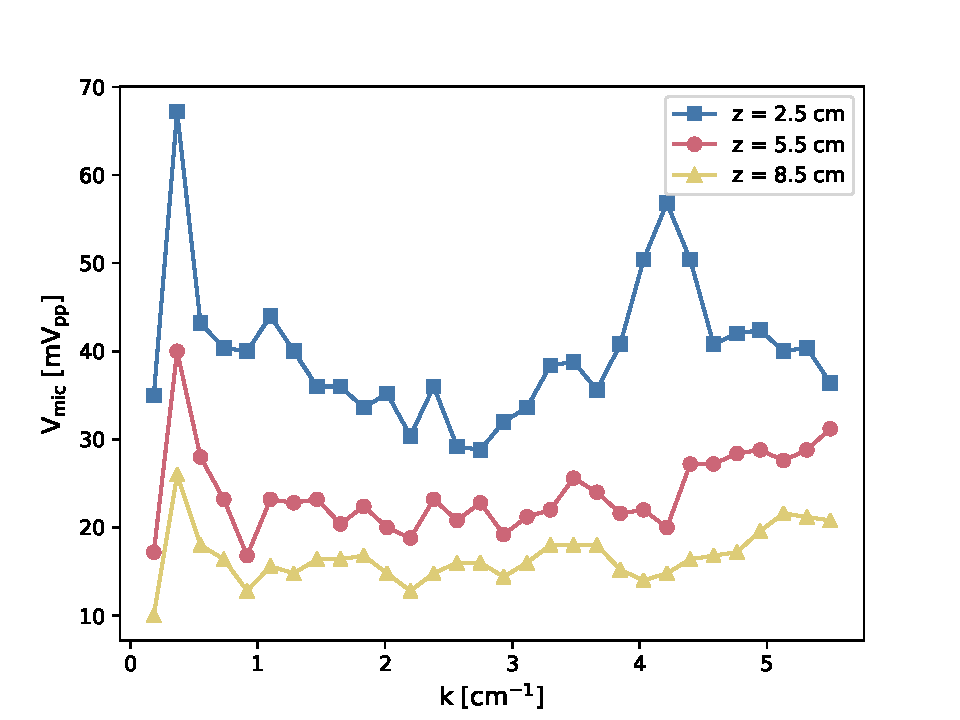
\includegraphics[width = \textwidth]{%
    Appendices/SoundWaveCharacterization/figs/tymphany_on_axis_amplitude.pdf}
  \caption[On-axis amplitude of sound waves]{%
    On-axis amplitude of sound waves as a function of
    wavenumber $k$ and height $z$ above the speaker face.
    Note that the amplitude is specified
    as a \emph{peak-to-peak} value.
  }
\label{fig:SoundWaveCharacterization:tymphany_on_axis_amplitude}
\end{figure}

\label{sec:SoundWaveCharacterization:Measurements:amlitude}
After centering the microphone on the speaker's symmetry axis,
the on-axis amplitude can be easily characterized by
varying both the frequency $f$ of the sound waves and
the microphone height $z$ above the speaker face.
The frequencies $f$ and heights $z$
are motivated by the parameters of the heterodyne interferometer
described in Chapter~\ref{ch:Implementation}.
Specifically, the interferometer spatial bandwidth
$|k| \leq \SI{5}{\per\centi\meter}$
from (\ref{eq:Implementation:kfsv_interferometer_design}) motivates
sound-wave measurements at frequencies
$f \lesssim \SI{30}{\kilo\hertz}$
(i.e.\ $|k| \lesssim \SI{5}{\per\centi\meter}$).
Further, to produce a robust interference signal
during sound-wave calibrations,
the speaker is placed very close
to the edge of the collimated probe beam,
which has 1/e $E$ radius $w_0 = \SI{3.4}{\centi\meter}$;
thus, sound-wave measurements are made at heights
spanning the probe-beam profile
$z
=
\{\SI{2.5}{\centi\meter}, \SI{5.5}{\centi\meter}, \SI{8.5}{\centi\meter}\}$.
The on-axis amplitude of the sound waves as a function of
wavenumber $k$ and height $z$ above the speaker face is shown in
Fig.~\ref{fig:SoundWaveCharacterization:tymphany_on_axis_amplitude}.
As expected, the on-axis amplitude decreases with
increasing distance $z$ from the speaker face.
Further, the on-axis amplitude has a complicated wavenumber dependence, but
it is relatively flat for
$\SI{1}{\per\centi\meter} \lesssim k \lesssim \SI{3.5}{\per\centi\meter}$.


\subsection{Wavefront phasing}
\label{sec:SoundWaveCharacterization:Measurements:phasing}
Characterizing the sound-wave phasing is somewhat more involved
than characterizing the on-axis amplitude,
as it requires measurements at several radial positions $\rho$
for each frequency $f$ and microphone height $z$.
For this reason, the wavefront-phasing measurements
are more coarsely sampled in frequency $f$
than the on-axis amplitude measurements in
Section~\ref{sec:SoundWaveCharacterization:Measurements:amlitude}.
For a given frequency $f$ and height $z$,
the sound-wave phasing is measured by
tracking a point of constant phase in the microphone waveform
as the radial position $\rho$ is varied;
such tracking can be easily accomplished
by triggering the oscilloscope
with a copy of the waveform that is driving the speaker.
To begin the radial scan,
the microphone height $z$ is selected, and
the microphone is displaced from the speaker's symmetry axis
by a few centimeters.
Then, in $\SI{1}{\centi\meter}$ increments,
the microphone is moved radially inwards towards the center;
upon passing through the center,
the radial scan is continued in $\SI{1}{\centi\meter}$ increments
until the sound-wave amplitude becomes negligible.
Note that beginning the radial scan
with a small displacement from the symmetry axis
allows empirical identification of the symmetry-axis location
(by e.g.\ fitting the measured amplitude and/or phasing
and identifying the extremum that occurs at the symmetry axis).

\begin{figure}
  \centering
  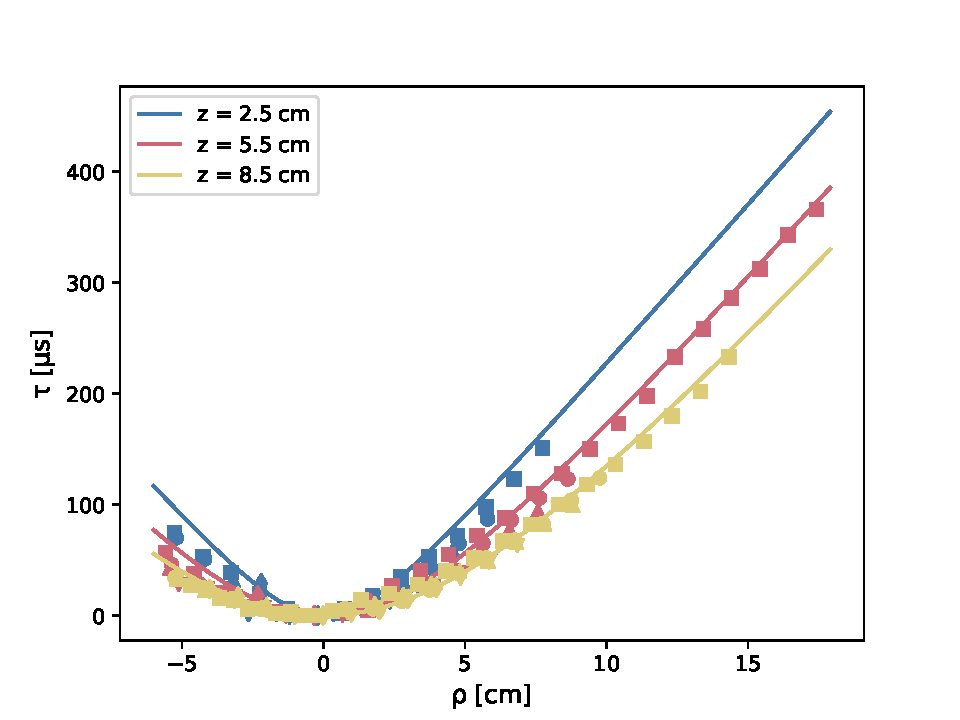
\includegraphics[width = \textwidth]{%
    Appendices/SoundWaveCharacterization/figs/tymphany_wavefront_phasing.pdf}
  \caption[Wavefront phasing of sound waves]{%
    Wavefront phasing of sound waves.
    The symbols show the measured time delay $\tau$
    between the wavefront at height $z$ and radial displacement $\rho$ and
    the corresponding on-axis wavefront (i.e.\ same $z$ but $\rho = 0$),
    with each symbol shape corresponding to particular frequency.
    The traces correspond to the time delay
    (\ref{eq:SoundWaveCharacterization:time_delay})
    predicted for spherical waves.
    The close proximity of the measured points to the spherical-wave traces
    indicates that, to lowest order, the waves are approximately spherical
    over the spatial domain and frequencies probed.
  }
\label{fig:SoundWaveCharacterization:tymphany_wavefront_phasing}
\end{figure}

At sufficiently large distances,
the speaker will behave like a point source,
producing sound waves with spherical wavefronts.
This point-source approximation is taken as a reasonable
starting point for the investigation of the wavefront phasing.
If a sound wave is measured on axis at height $z$ above the speaker,
the corresponding wavefront will subsequently arrive
at position $r = (z^2 + \rho^2)$
delayed by a time $\tau$
\begin{equation}
  \tau = \frac{r - z}{c_s},
  \label{eq:SoundWaveCharacterization:time_delay}
\end{equation}
where $c_s$ is the sound speed.
Fig.~\ref{fig:SoundWaveCharacterization:tymphany_wavefront_phasing}
compares the measured time delay to
the time delay predicted for spherical waves
(\ref{eq:SoundWaveCharacterization:time_delay})
as a function of height $z$, radial position $\rho$, and frequency $f$.
Clearly, to lowest order, the waves are approximately spherical
over the spatial domain and frequencies probed.


\subsection{Spatial envelope}
\label{sec:SoundWaveCharacterization:Measurements:envelope}
If the sound-wave amplitude is also measured
during the radial scans described in
Section~\ref{sec:SoundWaveCharacterization:Measurements:phasing},
the spatial envelope of the sound waves can also be quantified.
Fig.~\ref{fig:SoundWaveCharacterization:tymphany_spatial_envelope_z_5_5cm}
displays the spatial envelopes of sound waves of various frequencies $f$
at height $z = \SI{5.5}{\centi\meter}$ above the face of the speaker.
Clearly, the width of the spatial envelope decreases
with increasing frequency $f$.
Measurements at other heights $z$
exhibit qualitatively similar behavior.

\begin{figure}
  \centering
  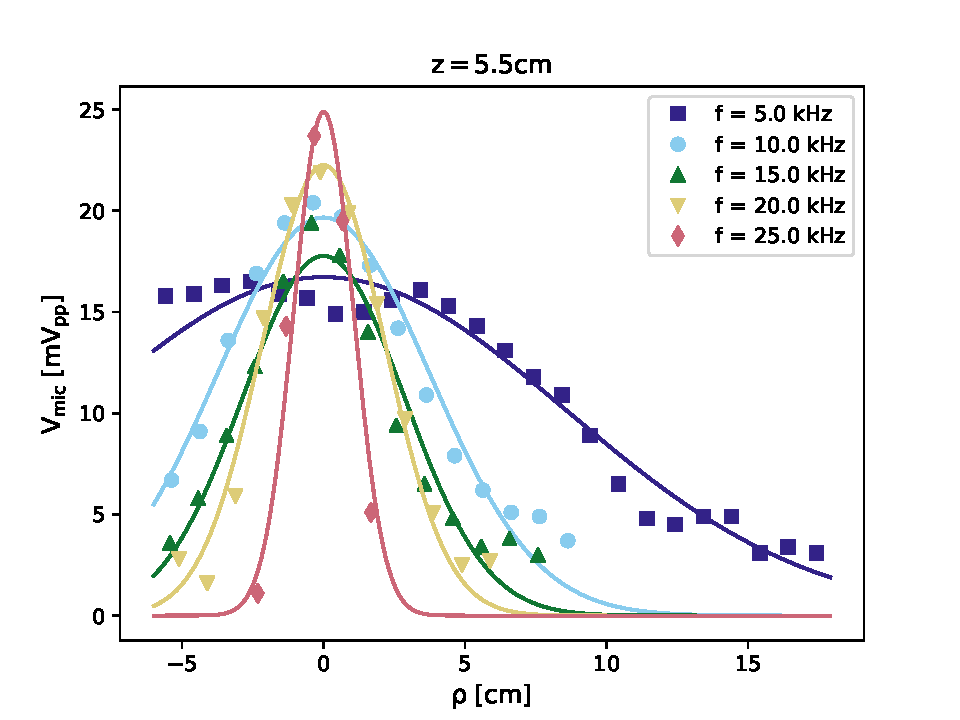
\includegraphics[width = \textwidth]{%
    Appendices/SoundWaveCharacterization/figs/tymphany_spatial_envelope_z_5_5cm.pdf}
  \caption[Representative spatial envelopes of sound waves]{%
    Sound-wave spatial envelopes for frequencies $f$
    at height $z = \SI{5.5}{\centi\meter}$ above the face of the speaker.
    Symbols indicate measurement points, while
    the traces correspond to Gaussian fits of the form
    (\ref{eq:SoundWaveCharacterization:Gaussian}).
    Measurements and fits at other heights $z$
    exhibit qualitatively similar trends.
  }
\label{fig:SoundWaveCharacterization:tymphany_spatial_envelope_z_5_5cm}
\end{figure}

The narrowing of the spatial envelope with increasing frequency
can be quantified by fitting the measurements
to an assumed functional form.
To lowest order, the spatial envelopes are well approximated by a Gaussian
\begin{equation}
  V_{\text{mic}}(\rho)
  =
  V_0(z, f)
  \exp\left[
    \frac{-\rho^2}{w(z, f)^2}
  \right],
  \label{eq:SoundWaveCharacterization:Gaussian}
\end{equation}
where $w(z, f)$ is the 1/e radius, which
is a function of the height $z$ and the sound-wave frequency $f$.
Gaussian fits to the envelope measurements are also shown in
Fig.~\ref{fig:SoundWaveCharacterization:tymphany_spatial_envelope_z_5_5cm}.
Deviations from a Gaussian are most apparent at low frequencies;
this may be attributable to baffle diffraction across the speaker face but
was not further investigated.
The approximation of a Gaussian envelope
will be sufficiently accurate for the present work.
Fig~\ref{fig:SoundWaveCharacterization:tymphany_gaussian_widths}
displays the fitted 1/e Gaussian radii $w$ as a function of
sound-wave wavenumber $k$ and
height $z$ above the face of the speaker.
As previously and anecdotally noted for $z = \SI{5.5}{\centi\meter}$,
the width of the spatial envelope $w$
decreases with increasing $k$ for each height $z$.
Further, $w$ increases with increasing $z$, which
results from free-space diffraction of the sound wave.

\begin{figure}
  \centering
  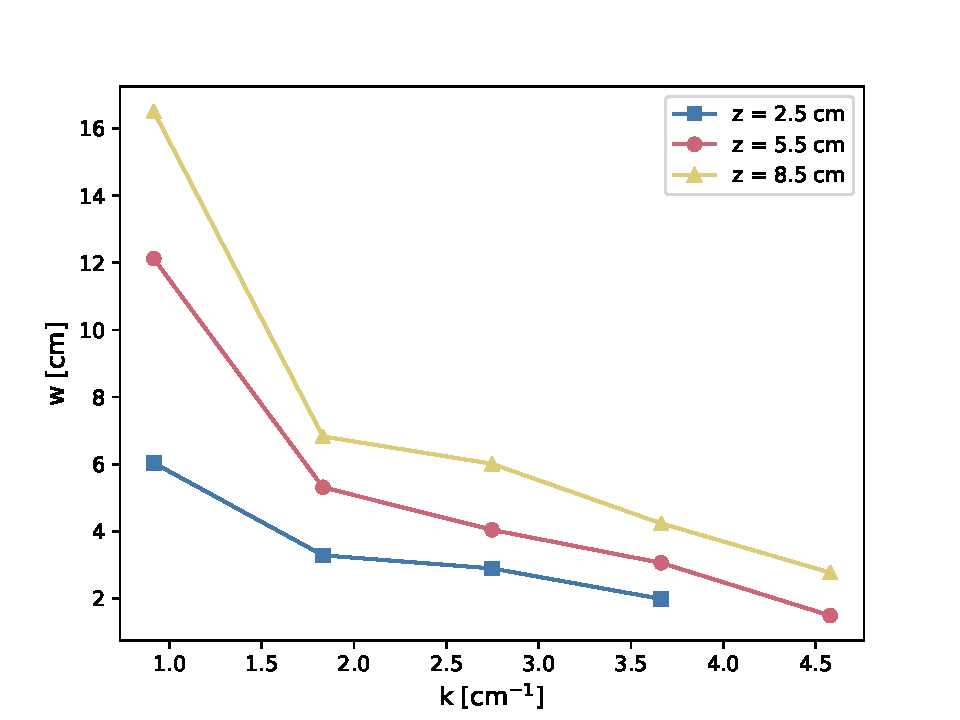
\includegraphics[width = \textwidth]{%
    Appendices/SoundWaveCharacterization/figs/tymphany_gaussian_widths.pdf}
  \caption[Gaussian widths of sound waves]{%
    Fitted 1/e Gaussian radii $w$ of sound waves
    as a function of sound-wave wavenumber $k$ and
    height $z$ above the face of the speaker.
  }
\label{fig:SoundWaveCharacterization:tymphany_gaussian_widths}
\end{figure}


\section{Sound-wave model}
\label{sec:SoundWaveCharacterization:Model}
Quantitatively predicting the response of a heterodyne interferometer
to sound-wave pressure fluctuations $\widetilde{p}(\vect{r}, t)$
requires knowledge of $\widetilde{p}$ at each point along the beam path.
Because the measurements described in
Section~\ref{sec:SoundWaveCharacterization:Measurements}
were made at discrete positions and frequencies,
it is necessary to develop an approximate \emph{model} of $\widetilde{p}$.
Recall that Section~\ref{sec:SoundWaveCharacterization:Measurements:phasing}
shows that the wavefronts of the sound waves
are approximately spherical, while
Section~\ref{sec:SoundWaveCharacterization:Measurements:envelope}
shows that the spatial envelope of the sound waves
is approximately Gaussian.
Thus, the sound-wave pressure fluctuation can be modeled as
\begin{equation}
  \widetilde{p}(\vect{r}, t)
  =
  \widetilde{p}_0(z, f)
  \cdot
  \exp\left[
    \frac{-\rho^2}{w(z, f)^2}
  \right]
  \cdot
  \cos(k r - \omega t),
  \label{eq:SoundWaveCharacterization:sound_wave_model}
\end{equation}
where
$z$ is the height above the speaker face,
$\rho = (x^2 + y^2)$ is the radial distance from the symmetry axis,
$\vect{r} = (x, y, z)$ is the spatial coordinate
relative to the center of the speaker face,
$r = |\vect{r}|$ is the corresponding distance
from the center of the speaker face,
$\omega$ is the angular frequency of the sound wave, and
$k$ is the wavenumber of the sound wave,
as determined from the sound-wave dispersion relation
(\ref{eq:SoundWaveCharacterization:sound_wave_dispersion_relation}).
Additionally, $\widetilde{p}_0(z, f)$ is the on-axis sound-wave amplitude, and
it is a complicated function of $z$ and $f$ that is computed
via radial-basis-function (RBF) interpolation
\cite[Sec.~3.7]{numerical_recipes}
\cite{scipy_radial_basis_function,radial_basis_function_stackoverflow}
of the measured on-axis amplitude shown in
Fig.~\ref{fig:SoundWaveCharacterization:tymphany_on_axis_amplitude}
(after conversion from $\SI{}{\volt}$ to $\SI{}{\pascal}$
using the absolute calibration of the microphone discussed in
Section~\ref{sec:SoundWaveCharacterization:Hardware:microphone}).
Similarly, $w(z, f)$ is the 1/e Gaussian radius of the sound wave, and
it is a complicated function of $z$ and $f$ that is computed
via RBF interpolation of the measured 1/e Gaussian radii shown in
Fig.~\ref{fig:SoundWaveCharacterization:tymphany_gaussian_widths}.
As an example,
a ``snapshot'' (i.e.\ at a single point in time) of the model's predicted
$\SI{15}{\kilo\hertz}$ pressure fluctuation $\widetilde{p}$ is shown in
Fig.~\ref{fig:SoundWaveCharacterization:model_pressure_field_15kHz}.

\begin{figure}
  \centering
  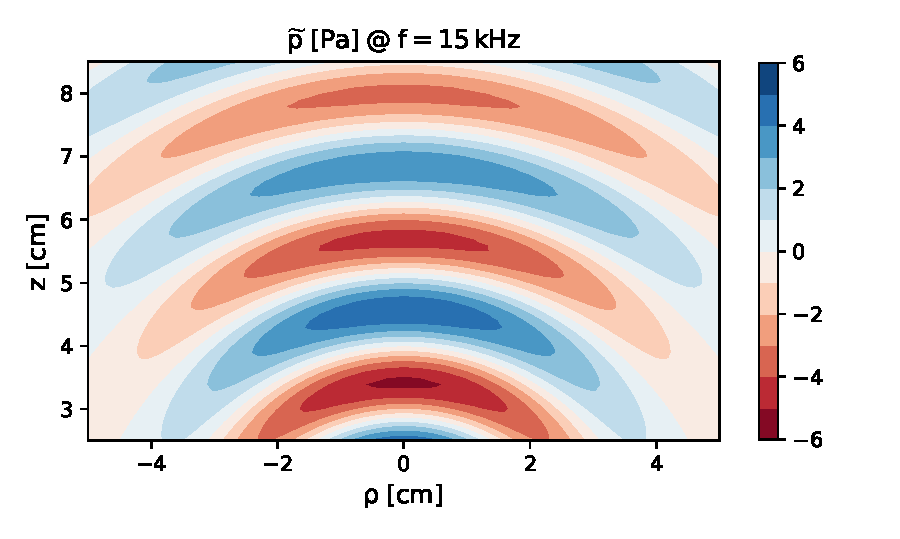
\includegraphics[width = \textwidth]{%
    Appendices/SoundWaveCharacterization/figs/model_pressure_field_15kHz.pdf}
  \caption[Snapshot of modeled pressure fluctuation]{%
    ``Snapshot'' (i.e.\ at a single point in time) of the model's predicted
    $\SI{15}{\kilo\hertz}$ pressure fluctuation $\widetilde{p}$.
  }
\label{fig:SoundWaveCharacterization:model_pressure_field_15kHz}
\end{figure}


\section{Perturbed index of refraction}
\label{sec:SoundWaveCharacterization:PerturbedIndexOfRefractiion}
Interferometric methods are sensitive to the index of refraction $N$.
Thus, quantitatively predicting the response of a heterodyne interferometer
requires computing the perturbed index of refraction $\tilde{N}$
corresponding to the sound-wave pressure fluctuation $\tilde{p}$
in (\ref{eq:SoundWaveCharacterization:sound_wave_model}).

While the quantification of air's refractive index
in the visible and infrared
has been vigorously pursued by the metrology community
\cite{young_refractivity_of_air, stone_index_of_refraction_of_air,
marchetti_ipt06, mathar_N_IR_07},
the lowest-order description will be sufficiently accurate
for the present application.
Specifically, an electromagnetic wave propagating through air
induces a time-varying polarization in the air
that alters the propagation of the wave;
it is precisely this interaction
that the refractive index $N$ quantifies.
Clearly, the induced polarization is
proportional to the number density $n$ of the air.
Thus, air's deviation from the vacuum refractive index of unity
is also proportional to $n$, i.e.\
\begin{equation}
  N - 1 = \alpha n,
  \label{eq:SoundWaveCharacterization:RefractiveIndex:deviation_from_vacuum}
\end{equation}
where $\alpha$ is a complicated function of
the atmospheric composition,
the vacuum wavelength of the electromagnetic wave, etc.
Explicitly writing the refractive index and number density
as sums of equilibrium and perturbed components
(i.e.\ $N = \bar{N} + \tilde{N}$ and
$n = \bar{n} + \tilde{n}$, respectively),
one readily sees that the perturbed refractive index can be written as
\begin{equation}
  \tilde{N}
  =
  \left( \frac{\bar{N} - 1}{\bar{n}} \right)
  \tilde{n}
  \label{eq:SoundWaveCharacterization:RefractiveIndex:perturbed_N_prelim}.
\end{equation}
Now, the sound-wave compressions and rarefactions
are approximately adiabatic such that
the total pressure $p$ and the total number density $n$ are related via
$p \propto n^{\gamma}$, where $\gamma$ is the ratio of specific heats.
Thus, the density perturbation $\tilde{n}$
corresponding to a sound-wave pressure perturbation
$|\tilde{p}| \ll \bar{p}$ (where $\bar{p}$ is the equilibrium pressure) is
\begin{equation}
  \tilde{n}
  \approx
  \left( \frac{\bar{n}}{\gamma \bar{p}} \right)
  \tilde{p}
\end{equation}
such that the perturbed refractive index
(\ref{eq:SoundWaveCharacterization:RefractiveIndex:perturbed_N_prelim})
becomes
\begin{equation}
  \tilde{N}
  \approx
  \left( \frac{\bar{N} - 1}{\gamma \bar{p}} \right)
  \tilde{p}.
  \label{eq:SoundWaveCharacterization:RefractiveIndex:perturbed_N}
\end{equation}
As \diiid\space sits very nearly at sea level,
the equilibrium pressure is $\bar{p} = \SI{101325}{\pascal}$.
Further, for dry air at $T \sim \SI{300}{\kelvin}$,
the ratio of specific heats is $\gamma = 1.4$, and
the deviation from the vacuum index of refraction
for $\SI{10.6}{\micro\meter}$ radiation is
$\bar{N} - 1 = 2.7 \times 10^{-4}$
\cite{marchetti_ipt06, mathar_N_IR_07, refractive_index_database}.
Thus, the perturbed refractive index
(\ref{eq:SoundWaveCharacterization:RefractiveIndex:perturbed_N})
for a $\SI{10.6}{\micro\meter}$ CO$_2$ probe beam becomes
\begin{equation}
  \tilde{N}
  \approx
  (1.9 \times 10^{-9})
  \,
  \tilde{p} \; [\text{Pa}].
  \label{eq:SoundWaveCharacterization:RefractiveIndex:perturbed_N_units}
\end{equation}


\section{Phase shift imparted to a CO2 probe beam}
\label{sec:SoundWaveCharacterization:PhaseShift}
A probe beam propagating through
a sound-wave pressure perturbation $\tilde{p}$
will acquire a phase shift
\begin{equation}
  \tilde{\phi}
  =
  k_0 \int \tilde{N} dl,
  \label{eq:SoundWaveCharacterization:phase_shift}
\end{equation}
where $k_0$ is the vacuum wavenumber of the probe beam,
$\tilde{N}$ is the perturbed index of refraction
(\ref{eq:SoundWaveCharacterization:RefractiveIndex:perturbed_N}), and
the integration is performed along the beam path.
This phase shift is, of course,
the measurable quantity of a heterodyne interferometer.
For a $\SI{10.6}{\micro\meter}$ CO$_2$ probe beam,
the phase shift (\ref{eq:SoundWaveCharacterization:phase_shift}) becomes
\begin{equation}
  \tilde{\phi} \, [\text{rad}]
  =
  (\SI{1.1e-5}{\per\centi\meter})
  \int
  (\tilde{p} \; [\text{Pa}])
  dl,
  \label{eq:SoundWaveCharacterization:phase_shift_units}
\end{equation}
where (\ref{eq:SoundWaveCharacterization:RefractiveIndex:perturbed_N_units})
has been referenced and
the differential path length $dl$ must have units of centimeters.
The variance of the phase shift imparted
by the sound-wave pressure fluctuation
(\ref{eq:SoundWaveCharacterization:sound_wave_model})
is shown in
Fig.~\ref{fig:SoundWaveCharacterization:phase_shift}.
To make a quantitative comparison
with the corresponding heterodyne-interferometer measurements,
the interferometer wavenumber response and noise floor
must also be accounted for;
such a comparison is performed in
Section~\ref{sec:Implementation:Calibration}.

\begin{figure}
  \centering
  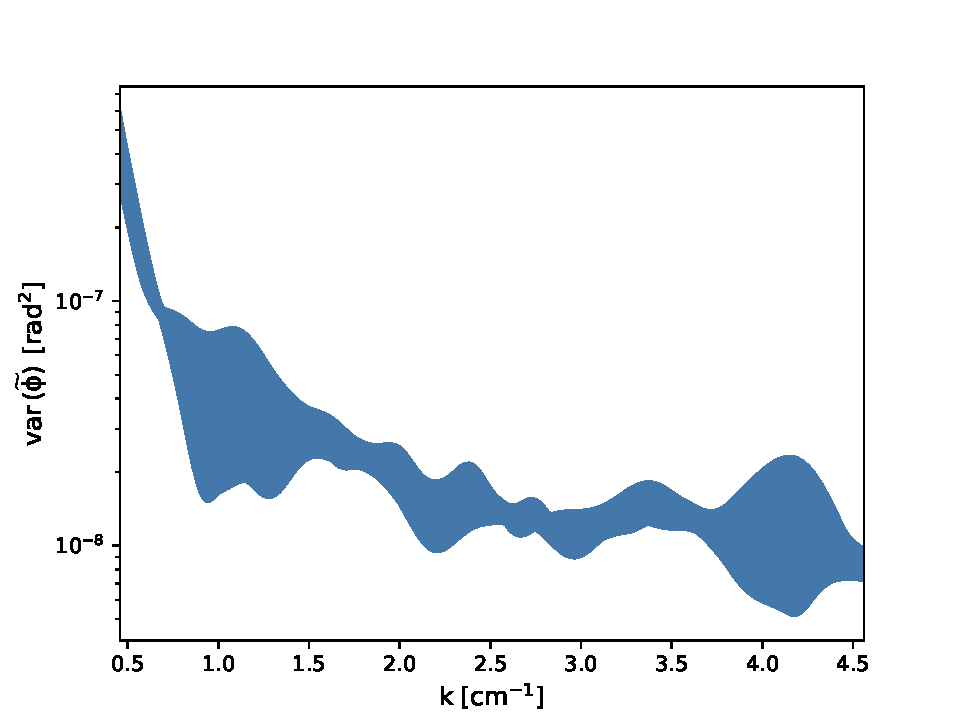
\includegraphics[width = \textwidth]{%
    Appendices/SoundWaveCharacterization/figs/model_phase_shift_to_CO2.pdf}
  \caption[Variance of phase shift imparted to a CO$_2$ probe beam]{%
    Variance of phase shift
    (\ref{eq:SoundWaveCharacterization:phase_shift_units})
    imparted to a $\SI{10.6}{\micro\meter}$ CO$_2$ probe beam
    by the sound-wave pressure fluctuation
    (\ref{eq:SoundWaveCharacterization:sound_wave_model}).
    Because the probe beam has finite cross section and
    the phase shift varies with the height $z$ above the speaker face,
    the maximum and minimum values of the variance
    are indicated by the upper and lower bounds of the shaded region,
    respectively;
    the minimum height considered is $z = \SI{2.5}{\centi\meter}$, and
    the maximum height considered is $z = \SI{8.5}{\centi\meter}$.
    The symmetry axes of the probe beam and the speaker
    are intersecting and orthogonal.
    To make a quantitative comparison
    with the corresponding heterodyne-interferometer measurements,
    the interferometer wavenumber response and noise floor
    must also be accounted for;
    such a comparison is performed in
    Section~\ref{sec:Implementation:Calibration}.
  }
\label{fig:SoundWaveCharacterization:phase_shift}
\end{figure}


\bibliographystyle{plainurl}
\bibliography{references}
